\section{Introduction}

In an epidemic, symptomatic cases are the predominant focus of treatment and usually represent the bulk of reported cases. 
However, infected individuals who are asymptomatic yet infectious can be a critical factor in the spread of some pathogens \citep{fraser2004factors}.
Asymptomatic individuals are hard to trace, unlikely to self-isolate, and are likely to retain normal social and travel patterns \citep{quilty2020effectiveness}.

There is significant ongoing interest in asymptomatic infections in COVID-19 \citep{chan2020familial, pan2020asymptomatic, tangearly} and their transmission potential \citep{bai2020presumed} for two major reasons.
First, the proportion of infections that are asymptomatic (see~\citep{mizumoto_2020}) is critical to attempts to estimate the likely burden of severe outcomes (including mortality \citep{fauci_nejm2020}) when the virus spreads through a population.
Second, understanding the possible role of \emph{transmission} by asymptomatic individuals is crucial to planning surveillance and control efforts \citep{fraser2004factors}.
Given that 86\% of the cases were undocumented (i.e., mildly symptomatic or asymptomatic) in Wuhan prior to travel restrictions and may account for 79\% of infection \DIFdelbegin \DIFdel{of }\DIFdelend \DIFaddbegin \DIFadd{in }\DIFaddend severe, symptomatic cases \citep{Lieabb3221}, asymptomatic cases are also likely to play an important role in the transmission of COVID-19.

Here, we focus on a third effect. 
If asymptomatic cases are important for transmission, they also have the potential to affect estimates of key parameters of disease spread such as the basic reproduction number ${\cal{R}}_0$ (i.e., the expected number of secondary cases generated by an average primary case in a fully susceptible population \citep{anderson1992infectious}). 
Thus, we investigate the relationship between individual-level features of asymptomatic cases (e.g., the probability that an infection is asymptomatic, asymptomatic case duration, transmission by asymptomatic individuals) to dynamics at the population scale.

\section{Methods}

We model viral spread using a renewal-equation framework \citep{heesterbeek1996concept}, which allows us to model the current incidence of infected individuals (i.e., the rate at which new infections occur in the population) as a function of previous incidence and how infectiousness of an infected individual varies over the course of their infection.
We divide incidence $i$ into two categories -- $i_a$ and $i_s$ -- corresponding to incidence of asymptomatic and symptomatic cases, respectively.
Newly infected individuals that are either asymptomatically or symptomatically infected can transmit the disease to others, but they \DIFaddbegin \DIFadd{may }\DIFaddend differ in their intrinsic reproduction numbers, ${\cal{R}}_a$ and ${\cal{R}}_s$, respectively, as well as intrinsic generation-interval distributions \citep{champredon2015intrinsic}, $g_a(\tau)$ and $g_s(\tau)$.
Generation intervals, which are defined as the time between when an individual is infected and when that individual infects another person \citep{svensson2007note}, \DIFdelbegin \DIFdel{depend on the }\DIFdelend \DIFaddbegin \DIFadd{shape the relationship between the epidemic growth rate $r$ and the reproduction number \mbox{%DIFAUXCMD
\citep{wallinga2007generation}}\hspace{0pt}%DIFAUXCMD
.
The differences in the generation-interval distributions between asymptomatic and symptomatic cases can be caused by the differences in the }\DIFaddend natural history of infection \DIFdelbegin \DIFdel{:
individuals with subclinical infections may have fast clearance and }\DIFdelend \DIFaddbegin \DIFadd{irrespective of their transmissibility:
Individuals with asymptomatic infections may recover faster and have }\DIFaddend short generation intervals, or \DIFaddbegin \DIFadd{have }\DIFaddend persistent infection and long generation intervals (cf. \citep{roberts2007model}).
\DIFdelbegin \DIFdel{The shape of the generation-interval distribution characterizes the relationship between the epidemic growth rate $r$ and the reproduction number \mbox{%DIFAUXCMD
\citep{wallinga2007generation}}\hspace{0pt}%DIFAUXCMD
.
}\DIFdelend 

Neglecting births and loss of immunity on the time scale of the outbreak, the dynamics of susceptibles and incidence are \DIFdelbegin \DIFdel{:
}\DIFdelend \DIFaddbegin \DIFadd{(see Table~S1 for parameter definitions):
}\DIFaddend \begin{eqnarray}
\dot{S}&=&-i(t)\DIFaddbegin \DIFadd{, }\DIFaddend \\
i(t)&=&\mathcal R_a S(t) \int_0^\infty i_a(t-\tau) g_a(\tau) \mathrm{d}\tau + \mathcal R_s S(t) \int_0^\infty i_s(t-\tau) g_s(\tau) \mathrm{d}\tau\DIFdelbegin \DIFdel{.
}\DIFdelend \DIFaddbegin \DIFadd{,
}\DIFaddend \end{eqnarray}
\DIFaddbegin \DIFadd{where $i(t) = i_a(t) + i_s(t)$.
}\DIFaddend The basic reproduction number of this system is:
\begin{equation}
{\cal{R}}_{0}= p {\cal{R}}_a + (1-p) {\cal{R}}_s,
\end{equation}
where $p$ is the proportion of \emph{incident cases} that are asymptomatic: $i_a(t) = p i(t)$.
The corresponding intrinsic generation-interval distribution of an average infected individual is given by: 
\begin{equation}
g(\tau) = z g_a(\tau) + (1-z) g_s(\tau),
\end{equation}
where we define the ``intrinsic'' proportion of asymptomatic transmission $z$ as the relative contribution of asymptomatic cases to the basic reproduction number:
\begin{equation}
z = p {\cal{R}}_a/{\cal{R}}_{0}.
\end{equation}
Note that the intrinsic proportion of symptomatic transmission satisfies
\begin{equation}
1-z = (1-p) {\cal{R}}_s/{\cal{R}}_{0}.
\end{equation}
Yet, this information is not sufficient to disentangle the role of asymptomatic cases, i.e., what fraction of secondary cases can be ascribed to \emph{realized} transmission from asymptomatic cases vs.~symptomatic cases?

The intrinsic proportion of asymptomatic transmission $z$ is a useful benchmark, but does not necessarily reflect the realized proportion of asymptomatic transmission, unless both types of infection have the same generation-interval distribution.
The \emph{realized} proportion of asymptomatic transmission, $q$ at time $t$ is given by:
\begin{equation}
\frac{q}{1-q}=\frac{\mathcal R_a S(t) \int_0^\infty i_a(t-\tau) g_a(\tau) \mathrm{d}\tau}{\mathcal R_s S(t) \int_0^\infty i_s(t-\tau) g_s(\tau) \mathrm{d}\tau}.
\end{equation}
During the period of exponential growth, we assume $S$ remains nearly constant, and $i(t)$ is proportional to $\exp(r t)$\DIFdelbegin \DIFdel{, and }\DIFdelend \DIFaddbegin \DIFadd{;
here, the observed exponential growth rate $r$ is an average of the exponential growth rates we would observe if there were only asymptomatic ($p=1$) or symptomatic ($p=0$) cases.
We then }\DIFaddend simplify by recalling that $i_a(t)= p i(t)$, $i_s(t)=(1-p)i(t)$ such that: 
\begin{equation}
\frac{q}{1-q}=\left(\frac{z}{1-z}\right)\frac{\delta_a}{\delta_s}.
\label{eq.qratio}
\end{equation}
Here, $\delta_c$ for each of the two classes is the average ``discount'' of a new infection -- the average relative contribution of a secondary infection to the epidemic, taking exponential growth into account:
\begin{equation}
	\delta_c = \int_0^\infty \exp(-r\tau) g_c(\tau) \mathrm{d}\tau.
\end{equation}
$\delta_c<1$ and grows smaller as the generation interval grows longer.
Thus, the realized proportion of asymptomatic infections will be increased (resp., decreased) if transmission is relatively faster (slower) along the asymptomatic route.
The discount $\delta$ also depends on the relative variation in the generation-interval distribution, the ``dispersion'': \DIFdelbegin \DIFdel{more }\DIFdelend \DIFaddbegin \DIFadd{More }\DIFaddend variation in generation intervals leads to more opportunities for fast spread and thus to higher values of $\delta$ (similar to shorter average generation intervals). 

To estimate the effects of assumptions about asymptomatic transmission on the \DIFaddbegin \DIFadd{inferred }\DIFaddend importance of asymptomatic transmission and estimates of the basic reproduction number ${\cal{R}}_0$, we parameterize the generation interval distributions of asymptomatic and symptomatic cases based on their means, $\bar G_a$ and $\bar G_s$, and dispersions, $\kappa_a$ and $\kappa_s$.
We assume that generation intervals are gamma distributed, and we set the dispersion to be equal to the squared coefficient of variation (the reciprocal of the gamma shape parameter, see Supplementary Materials).
We assume that epidemic growth rate $r$ and the generation-interval distribution of symptomatic case are known, using parameter values that are consistent with earlier COVID-19 models \citep{park_preprint}: $1/r=7$ days, $\bar G_s=8$ days, and $\kappa_s=0.5$.
We infer values of $q$ using Eq.~\req{eq.qratio} and ${\cal{R}}_0$ using the Euler-Lotka equation \citep{lotka1907relation}:
\begin{equation}
\frac{1}{\mathcal R_0} = \int \exp(-r \tau) \DIFaddbegin \left(\DIFadd{z }\DIFaddend g\DIFaddbegin \DIFadd{_a}\DIFaddend (\tau) \DIFaddbegin \DIFadd{+ (1-z) g_s(\tau)}\right) \DIFaddend \mathrm{d} \tau.
\end{equation}
\DIFaddbegin \DIFadd{We compare this with the naive estimate of the basic reproduction number that assumes that the generation-interval distributions of the asymptomatic and symptomatic cases are identical:
}\begin{equation}
\DIFadd{\frac{1}{\mathcal R_{\tiny \textrm{naive}}} = \int \exp(-r \tau) g_s(\tau) \mathrm{d} \tau.
}\end{equation}
\DIFaddend In Supplementary Materials, we also use an ordinary differential equation model \DIFaddbegin \DIFadd{(SEIR model) }\DIFaddend including both asymptomatic and symptomatic cases to give a concrete example of how differences in generation intervals affect both $q$ and estimates of $\mathcal R_0$.

\section{Results}

\begin{figure*}[b!]
\begin{center}
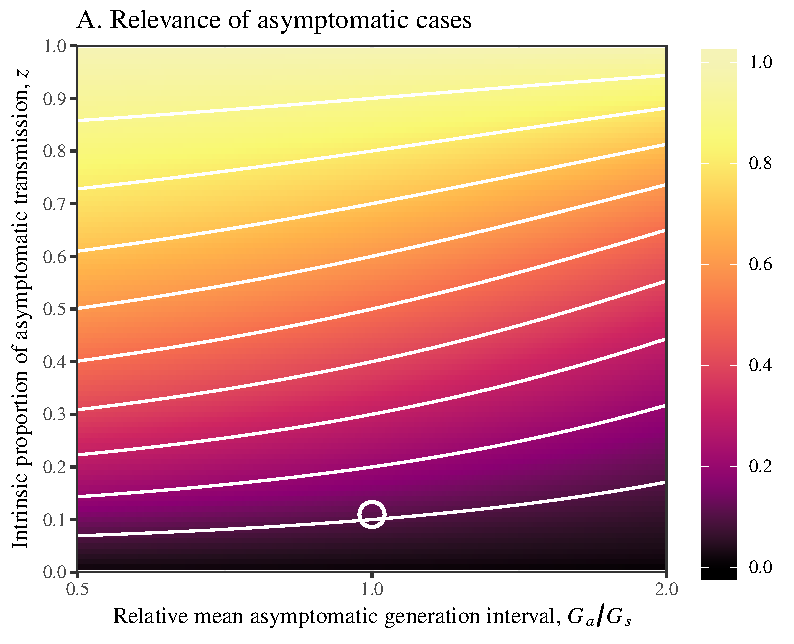
\includegraphics[width=0.45\textwidth]{figheatmap.pdf}
\mbox{\hspace{0.05\textwidth}}
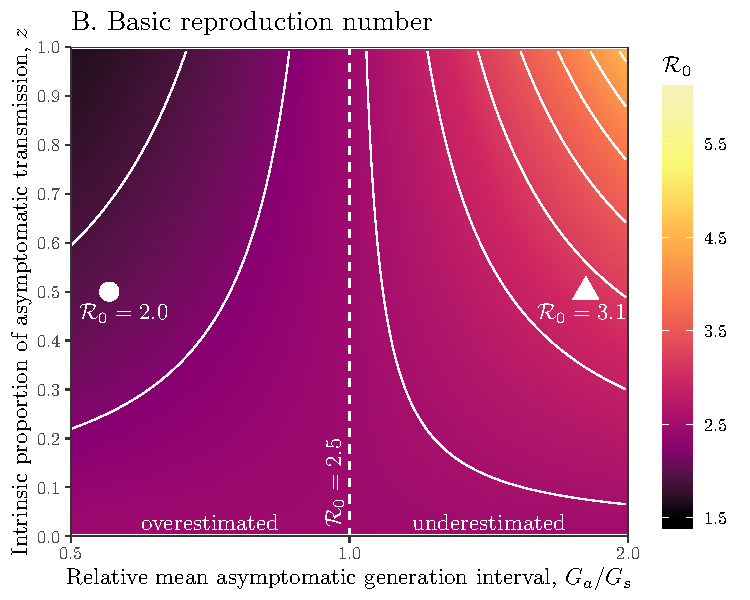
\includegraphics[width=0.45\textwidth]{figheatmap_R0.pdf}
\caption{Effects of intrinsic proportion of asymptomatic transmission on the realized proportion of asymptomatic transmission and basic reproduction number, given variation in
the mean generation interval of asymptomatic cases. 
(A) Increasing the speed of asymptomatic transmission (shorter generation intervals) increases the realized proportion of asymptomatic transmission, $q$.
(B) Increasing the speed of asymptomatic transmission (shorter generation intervals) decreases the basic reproduction number ${\cal{R}}_0$.
When $\bar G_a$ is smaller (larger) than $\bar G_s$, estimates based on the observed generation distribution for symptomatic cases (${\cal{R}}_0=2.5$; dashed line) are expected to over- (under-) estimate the true $\mathcal R_0$.
\DIFdelbeginFL \DIFdelFL{Triangle }\DIFdelendFL \DIFaddbeginFL \DIFaddFL{For both panels, the circle }\DIFaddendFL denotes $z=0.5$ and $\bar G_a/\bar G_s = 0.55$ \DIFdelbeginFL \DIFdelFL{.
Circle }\DIFdelendFL \DIFaddbeginFL \DIFaddFL{whereas the triangle }\DIFaddendFL denotes $z=0.5$ and $\bar G_a/\bar G_s = 1.8$.
Solid lines show contours for $q$ and \Ro\ values. 
\DIFaddbeginFL \DIFaddFL{The dashed line represents the naive estimate that assumes $\bar G_a = \bar G_s$.
}\DIFaddendFL Here, we assume $1/r=7$ days, $\bar G_s=8$ days, and $\kappa_s=\kappa_a=0.5$.
\label{fig.importance}}
\end{center}
\end{figure*}

We explore the effects of different assumptions about speed and effectiveness of asymptomatic transmission on the importance of asymptomatic transmission and estimates of the basic reproduction number ${\cal{R}}_0$, using a gamma assumption (see Methods).
Across the range of parameters we explore, the intrinsic proportion of asymptomatic transmission $z$ is similar to the realized proportion $q$ (Figure~\ref{fig.importance}A).
As the relative mean generation interval of asymptomatic transmission, $\bar G_a/\bar G_s$, increases, $q$ decreases because symptomatic cases are more likely to have short generation intervals\DIFdelbegin \DIFdel{(i.e., fast transmission events), }\DIFdelend \DIFaddbegin \DIFadd{, }\DIFaddend which drive the spread during the growth phase (Figure~\ref{fig.importance}A).
\DIFaddbegin \DIFadd{In Figure~S1, we present the same figure but showing differences between the realized and the intrinsic proportion of asymptomatic transmission, $q-z$.
}\DIFaddend 

Figure~\ref{fig.importance}B shows the effect of different assumptions about the generation interval of asymptomatic cases, $\bar G_a$, on the \DIFaddbegin \DIFadd{estimated }\DIFaddend basic reproduction number ${\cal{R}}_0$.
When $\bar G_a$ is long compared to $\bar G_s$, then we are effectively assuming a longer mean for the overall generation interval. 
This assumption leads to a larger estimate of \Ro\ for a fixed value of $r$ (see~\citep{park_2019practical}).
Conversely, when $\bar G_a < \bar G_s$, generation intervals are shorter, leading to lower estimates of the epidemic strength \Ro. Both of these effects are stronger when the intrinsic proportion of asymptomatic transmission $z$ increases (and disappear as $z\to0$).
Therefore, when ${\cal{R}}_0$ is estimated without explicitly accounting for asymptomatic spread (white, dashed line in Figure~\ref{fig.importance}B), it can be over- or under- estimated depending on the relative duration of infection between symptomatic and asymptomatic individuals.
The qualitative effects of $z$ and $\bar G_a/\bar G_s$ on $q$ and ${\cal{R}}_0$ remain robust when we assume narrower ($\kappa_s = \kappa_a = 0.3$; Figure~\DIFdelbegin \DIFdel{S1}\DIFdelend \DIFaddbegin \DIFadd{S2}\DIFaddend ) or wider ($\kappa_s = \kappa_a = 0.8$; Figure~\DIFdelbegin \DIFdel{S2}\DIFdelend \DIFaddbegin \DIFadd{S3}\DIFaddend ) generation intervals.

Relative generation-interval dispersion of asymptomatic cases $\kappa_a/\kappa_s$ have similar, but smaller, effects on $q$ and ${\cal{R}}_0$ (Figure~\DIFdelbegin \DIFdel{S3}\DIFdelend \DIFaddbegin \DIFadd{S4}\DIFaddend ).
Since a wider generation-interval distribution has a higher proportion of early transmission than a narrow one, increasing the generation-interval dispersion has qualitatively similar effects on $q$ and ${\cal{R}}_0$ as decreasing the mean generation interval.

\section{Discussion}

Much is still unknown about the time scale and effectiveness of asymptomatic transmission in COVID-19.
Here we highlight the need to characterize the generation-interval distribution for asymptomatic transmission, and its consequences not only for contact tracing but for estimation of the basic reproduction number of the ongoing COVID-19 outbreak~\citep{park_preprint} and of the effective proportion of asymptomatic transmission during the exponential-growth phase.
Our reproductive number findings fit into a broader framework linking epidemic speed, strength, and generation intervals -- for a given observed speed increases in the mean generation interval imply larger reproduction number~\citep{wearing2005appropriate, roberts2007model, wallinga2007generation, powers2014impact, park_2019practical}.

If asymptomatic infections are more persistent than symptomatic ones, the mean generation interval for COVID-19 could be longer than estimated from symptomatic cases alone -- possibly \DIFdelbegin \DIFdel{increasing }\DIFdelend \DIFaddbegin \DIFadd{causing }\DIFaddend ${\cal{R}}_0$ \DIFaddbegin \DIFadd{to be underestimated }\DIFaddend (Figure~\ref{fig.importance}B).
However, if asymptomatic cases tend to resolve quickly, then current estimates of ${\cal{R}}_0$ may be over-estimates of the underlying strength (Figure~\ref{fig.importance}B), and asymptomatic cases may be driving a larger fraction of secondary cases than we would expect without accounting for their differences (Figure~\ref{fig.importance}A)\DIFaddbegin \DIFadd{.
The importance of these effects depends on the relative infectiousness of asymptomatic transmission as well as the proportion of incident cases that are asymptomatic (and therefore the intrinsic proportion of asymptomatic transmission $z$.
The biases in the estimates of ${\cal{R}}_0$ will necessarily bias estimates of the amount of intervention required to control the epidemic}\DIFaddend .
Note that cases do not have to be completely asymptomatic for our qualitative results to apply.
People with mild symptoms unlikely to be diagnosed in a particular time and place (sometimes referred to as subclinical cases) are expected to affect transmission patterns in the same way.

We focus here on the exponential phase, so it is worth noting that the realized proportion of asymptomatic transmission $q$ is time-dependent, varying with dynamic changes in incidence and proportion susceptible. 
Future work might also consider the ways in which asymptomatic individuals can modulate the catalysis of epidemics in a networked metapopulation~\citep{watts_pnas2005, chinazzi2020effect, du2020risk}.
Characterizing the role of asymptomatic individuals in driving the persistence of the epidemic will be critical for assessing the post-pandemic outcome \citep{lipsitch_preprint}.
